
In this chapter we present the methodology that we are proposing for
learning chunks of good designs. We give the multi-objective formulation
for the the brush-less DC permanent magnet motor design problem which was
discussed in section \ref{expertInAction} earlier, and apply our procedure
on this problem as we elucidate each step.  The brush-less DC permanent
magnet design problem was first analyzed in \citep{chidam99} as discrete
optimization problem to illustrate catalog-based customization. The same
problem was analyzed in \citep{deb08} to discover innovative design
principles from the optimization results. We borrow the same problem
formulation as in \citep{deb08} for our study.

\section{Overview of the chunking process}
Figure \ref{overview} shows the steps of our proposed chunking process. The
first stage in the process is obtaining a set of optimal solutions using
multi-objective optimization. The second step is the manifold estimation of
the optimal solutions obtained in the first step. The next step, clustering
the optimal solutions, is the most important step in chunking procedure. In
this step the optimal solutions are clustered using a density based
partitioning algorithm in the combined objective-parameter space
space. Finally we model the clusters into manifolds which represent the
chunks of similar optimal solutions.
 
\begin{figure}[ht]\begin{center}
 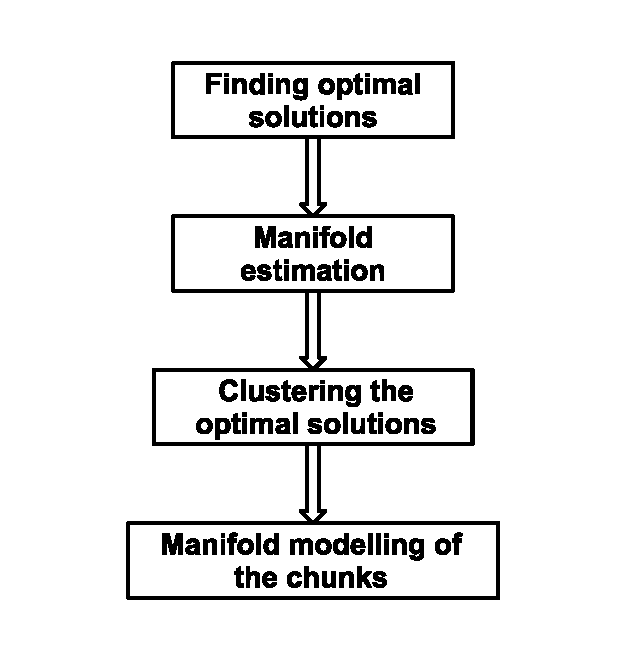
\includegraphics[width=75mm, height=75mm]{dia/overview.eps}
 \caption{Overview of the chunking process.}
 \label{overview}
\end{center}\end{figure}



\section{Obtaining set of optimal designs}
Since we want to learn chunks of ``good" solutions we must have a way of
characterising good solutions. In context of design, only the best possible
designs may be considered as good, a designer who produces feasible but
sub-optimal designs can not be called an expert. A human designer during
her routine exploration of a design problem comes across some designs that
are superior to all others. These are the designs that she is more likely
to retain in her memory as a chunk. In effect, she is searching for optimal
designs which when found are retained. The first step of our procedure to
learn patterns of good designs is to obtain a representative set of such
optimal designs.  In this section, we discuss the possible techniques of
obtaining such representative optimal solutions set.

\subsection{Conventional multi-objective optimization techniques}
In classical multi-objective optimization techniques the objectives are
combined to form one single objective using some knowledge of the problem
being solved. The optimization of the single objective-results in a single
pareto-optimal solution.

One of the classical methods of multi-objective optimization is the method
of objective weighting \citep{deb01,deb94}.  Multiple objectives are
combined into an overall objective by assigning fractional weights to the
individual objective functions which sum to one. The optimal solution is
controlled by the weight vector.

In the method of distance functions, the single objective is derived from
multiple objectives using a demand level vector $\overline{\textbf{y}}$ as
follows:\\
\begin{align}
  Z = \left[ \displaystyle\sum\limits_{i=1}^N {|f_i(\textbf{x} - \overline{y_i})|}\right] ^{1/r}, \quad &1 \leqslant r < \infty 
\end{align}\\
where $\textbf{x} \in \textbf{X}$, the feasible region. An arbitrary demand
level vector may result in a objective that doesn't have an optimal
solution, hence the decision maker must have a thorough knowledge of
individual optima of the objectives prior to the selection of the demand
level vector.

The Min-Max formulation method is different in principle from the above two
methods in that it attempts to minimize the relative deviations from the
individual optima, that is to say, it tries to minimize the objective
conflict.

The most important drawback of these classical multi-objective optimization
methods with respect to our objective is that they yield only one
pareto-optimal solution in a single run. Secondly, all of them require some
knowledge of the problem, such as the weight vector or demand
vector. Moreover it is not possible to find all pareto-optimal solutions in
some non-convex multi-objective optimization problems.

\subsection{Evolutionary algorithms for multi-objective optimization}
Evolutionary approaches to multi-objective optimization are much more
suited to the purpose of generating a representative optimal solution set,
as they can search the solution space in parallel for optimal solutions,
and produce a set of pareto-optimal solutions in a single run.

Evolutionary algorithms try to mimic the process of natural selection,
whereby only the specimens most adapted to the environment survive and
evolve. All the algorithms start with randomly chosen population of
feasible solutions and search and reproduce the best solutions in the
population. This search and reproduce procedure is repeated for many
generations, until the next generation doesn't result in significant
improvements. The first practical evolutionary multi-objective optimization
algorithm was the Vector Evaluated Genetic Algorithm (VEGA)
\citep{schaffer85}. One of the problems with VEGA is its bias towards some
pareto-optimal solutions. A non-dominated sorting procedure was proposed by
Goldberg to overcome this drawback, in which a ranking selection method is
used to emphasize good points and a niche method is used to maintain stable
sub-populations of good points.  One algorithm that that implements this
non-dominated sorting procedure is the NSGA \citep{deb94}.

This algorithm was further improved upon, and a new algorithm NSGA-II
\citep{deb02} was proposed which had better and faster convergence towards
the true pareto-front due to a fast non-dominated sorting approach. Since
it was first proposed, the NSGA-II has found application in a wide variety
of engineering optimizations and design problems. Several studies have been
published illustrating the versatility of NSGA-II in a wide variety of
situations. All these advantages that NSGA-II has over other algorithms,
and its proved versatility make it an ideal candidate for the purpose of
generating a set of pareto-optimal solutions

\subsection{The BDCPM motor design problem}
We now introduce the mulit-objective optimization formulation for the BDCPM
(brush-less DC permanent magnet motor) design problem and derive a set of
pareto-optimal solutions using NSGA-II. A BDCPM motor comprises of an outer
stator assembly with windings on a frame and inner rotor assembly having
permanently mounted magnets, shown in Figures \ref{bdcpmStator} and
\ref{bdcpmRotor}. Several variants of this basic design exist. The original
study \citep{chidam99} considered 24 slots 4 pole machine.


\subsubsection{The multi-objective optimization problem}
Figure \ref{bdcpmRotor} shows the rotor assembly of a BDCPM motor. A
ring-magnet is bonded onto a stepped shaft that fits in the bore of the
stator assembly. The total length of the motor is $L_{sh}$. The shaft
length is equal to the sum of stack length and the side clearances, $
L_{sh} = L + 2L_{cl}$. The side clearance values $L_{cl}$, and other parameters for
different lamination types are listed in Table
\ref{ltypeDimTable}.

\begin{figure}[ht]\begin{center}
 \fbox{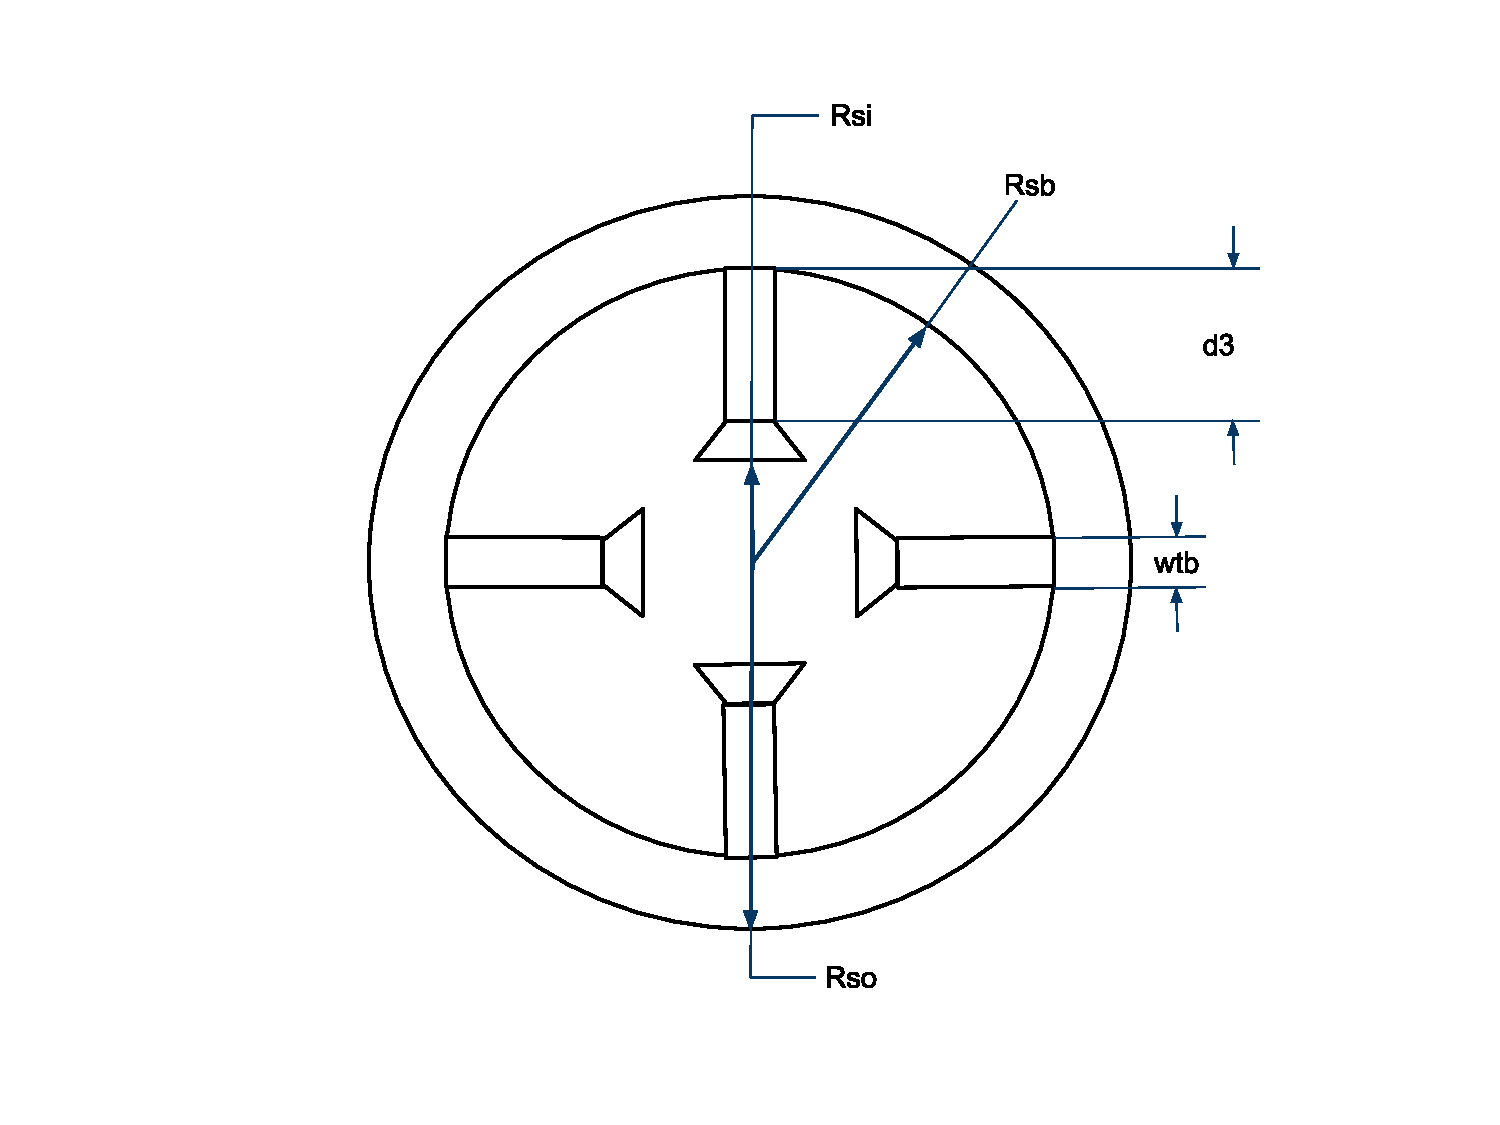
\includegraphics[width=88mm, height=65mm]{dia/bdcpmStator.eps}}
 \caption{BDCPMM Stator assembly.}
 \label{bdcpmStator}
\end{center}\end{figure}

\begin{table}[!ht]
  \centering
  \begin{tabular}{|c|c|c|c|c|c|c|c|}
    \hline
    $L_{type}$ & $R_{si}$ (mm.) & $d_3$ (mm.) & $w_{tb}$ (mm.) & $w_{bi}$ (mm.) & $L_{cl}$ (mm.)& $R_{sh}$ (mm.) & $R_{st}$ (mm) \\
    \hline
    X & 21.90 & 12.0 & 2.39 & 5.23 & 4.215 & 4.11 & 0.016 \\
    \hline
    Y & 22.22 & 15.1 & 2.39 & 5.23 & 4.265 & 4.11 & 0.016 \\
    \hline
    Z & 25.40 & 15.1 & 2.80 & 5.50 & 4.775 & 4.45 & 0.019 \\
    \hline
  \end{tabular}
  \caption{Dimensions of the BDCPM motor family}
  \label{ltypeDimTable}
\end{table}

\begin{figure}[ht]\begin{center}
 \fbox{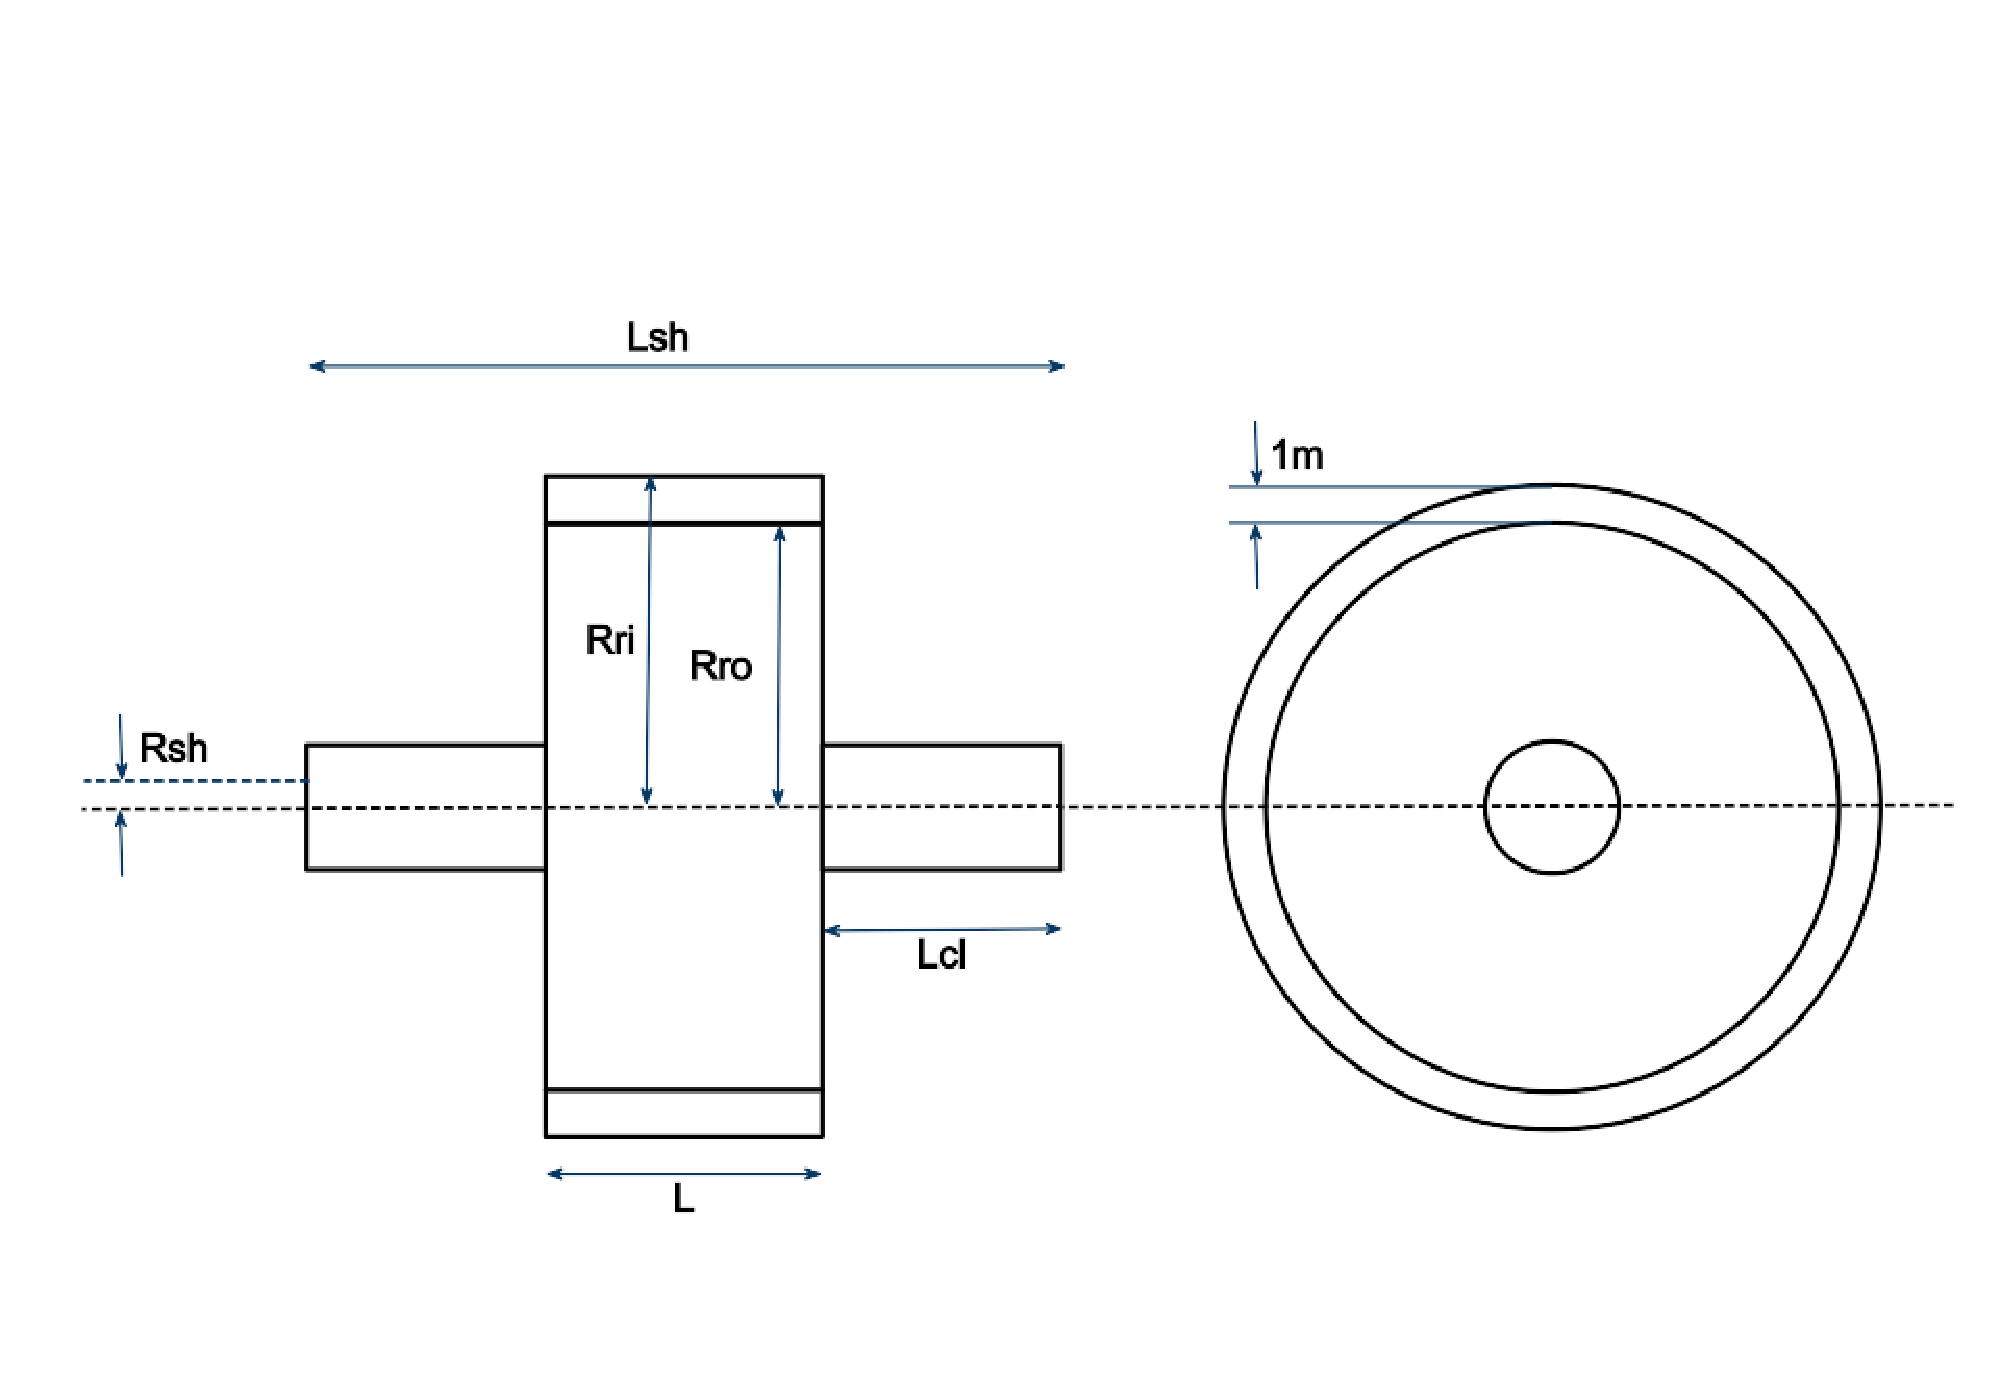
\includegraphics[width=83mm, height=59mm]{dia/bdcpmRotor.eps}}
 \caption{BDCPMM Rotor Assembly.}
 \label{bdcpmRotor}
\end{center}\end{figure}

Five design variables are considered for the design process, other design
parameters are fixed to values that are convenient for the
manufacturer. The design variables are:

\begin{enumerate}
\item Number of laminations $n_l \in [44, 45,\dots ,132]$
  
\item Number of turns in each coil  $N \in [20, 21, \dots, 80]$

\item $L_{type} \in [\textsf{X, Y, Z}]$ is one of the three types of 
laminations allowed to build the motor

\item $M_{ph} \in [Y, \Delta ]$ is one of the two types of elctric 
connections and

\item $A_{gauge} \in [16, 16.5, 17, \dots , 23.5]$ is one of the 16 
wire gauges used in the windings.
\end{enumerate}

All the design variables are discrete in nature, of which $L_{type}$ 
and $M_{ph}$ take 3 and 2 values respectively. $n_l$ and $N$ are 
integer valued variables while $A_{gauge}$ takes 16 equally spaced 
values in its domain.

The cost expression for the first objective includes the material and
estimated production cost. Each term in the expression is obtained from the
regression analyses of data obtained from practice. The detailed procedure
discribing the derivation of the cost terms and torque expressions can be
found in \citep{chidam99}.

The actual multi-objective optimization problem is formulated as follows:

%%%%%Cost function begins here%%%%%


\begin{singlespacing}

\begin{flushleft}



Minimize:   \\
$ C_{total} (n_{l}, N, L_{type}, M_{ph}, A_{wire}) = 
\begin{cases}
\quad 2.6(\frac{n_{l}}{44})^{0.25}, & \text{for $L_{type} =$ \textbf{X}} \\
\quad 0.38 + 2.42(\frac{n_{l}}{44})^{0.37}, & \text{for $L_{type} =$ \textbf{Y}} \\
\quad 1.07 + 1.83(\frac{n_{l}}{44})^{0.58}, & \text{for $L_{type} =$ \textbf{Z}} 
\end{cases} $ \\

$
+  [ \left\{0.026, 0.028, 0.03\right\}n_{l} \cong L_{type} = \{ \textbf{X}, \textbf{Y}, \textbf{Z} \} $\\
$
\, + \, \dfrac{n_{l}}{44} \, + \,   9.8 \times 10^{5} A_{wire} N [ 5.8  \times  10^{-4} n_{l}
   +  \dfrac{\pi}{2} \{ w_{tb} + \dfrac{5\pi}{12}(R_{si} + \dfrac{d_{3}}{2}) \}]
$ \\

$
+ \, 0.3035 \, + \, 0.876 N [ 5.8 \times 10^{-4} n_{l} \, + 
 \dfrac{\pi}{2} \{ w_{tb} \, + \, \dfrac{5 \pi}{12}(R_{si} \, + \, \dfrac{d_{3}}{2})\}]
$\\

$
\, + \, \pi \left[ \left\{ 31.2( R_{si} + d_{3} + w_{bi}) + 0.0312 \right\} \left\{ L_{sh} - 5.08 \times 10^{-3} \right\} \right]
$\\
$
\, + \, 
\begin{cases}
\quad 0.7(\frac{5.8 \times 10^{-4} n_{l} + 0.0792}{0.1047})^{1.21},  & \text{for $L_{type} = $ \textbf{X}} \\
\quad 0.54 + 0.26( \frac{5.8 \times 10^{-4} n_{l} + 0.0802}{0.1057})^{3.74}, & \text{ for $L_{type} =$ \textbf{Y}} \\
\quad 0.58 + 0.32( \frac{5.8 \times 10^{-4} n_{l} + 0.0905}{0.1160})^{4.23}, & \text{ for $L_{type} =$ \textbf{Z}} \\
\end{cases}
$\\
$ \, + \, 9 \, + \, \begin{cases}
\quad 1.3(\frac{5.8 \times 10^{-4} n_{l} + 0.0792}{0.1047})^{0.38} (\frac{n_{l}}{44})^{0.18}, & \text{for $L_{type} =$ \textbf{X}} \\
\quad 1.6(\frac{5.8 \times 10^{-4} n_{l} + 0.0802}{0.1057})^{0.38} (\frac{n_{l}}{44})^{0.40}, & \text{for $L_{type} =$ \textbf{Y}} \\
\quad 1.8(\frac{5.8 \times 10^{-4} n_{l} + 0.0905}{0.1160})^{0.41} (\frac{n_{l}}{44})^{0.52}, & \text{for $L_{type} =$ \textbf{Z}}
\end{cases}
$\\
$
\, + \, (1.536 R_{st} - 6.26 \times 10^{-3}) n_{l} \, + \, (2.014 R_{si} \, - \, 8.21 \times 10^{-3}) n_{l}
$\\
$
\, + \, \pi \{29.4(R_{si} - 7.25 \times 10^{-3})^{2} n_{l} \, + \, 1.014 \times 10^{5} R_{sh}^{2} L_{cl}\} 
$\\
$
\, + \, 0.1862 \, + \, 5.31 \times 10^{4} \pi [ R_{st}^{2} L_{st} \, - \,  2 R_{sh}^{2} L_{cl} 
\, - \, 5.8 \times 10^{-4} n_{l}(R_{si} - 7.25 \times 10^{-3})^{2}] 
$\\
$
 \, + \, 0.01 \, + \,0.1473 \pi (R_{si} - 7.25 \times 10^{-3}) n_{l} \, + \, \begin{cases}
\quad 1.2, & \text{for $T_{p} \le 3.5$} \\
\quad 1.6, & \text{for $T_{p} > 3.5$} 
\end{cases}
$\\
$
\, + \, \left[ \left\{ 0.5, 0.55, 0.60 \right\} \cong L_{type} = \{ \textbf{X}, \textbf{Y}, \textbf{Z} \} \right]
$\\
$
\, + \, \begin{cases}
\quad 3.2(\frac{5.8 \times 10^{-4} n_{l} + 0.0792}{0.1047})^{-1.92}(\frac{n_{l}}{44})^{0.92}, & \text{for $L_{type} = $ \textbf{X}} \\ 
\quad 3.4(\frac{5.8 \times 10^{-4} n_{l} + 0.0802}{0.1057})^{-1.92}(\frac{n_{l}}{44})^{1.06}, & \text{for $L_{type} = $ \textbf{Y}} \\ 
\quad 3.7(\frac{5.8 \times 10^{-4} n_{l} + 0.0905}{0.1160})^{-3.25}(\frac{n_{l}}{44})^{1.60}, & \text{for $L_{type} = $ \textbf{Z}} 
\end{cases}
$
\\[\baselineskip]

%%%%Torque function%%%%

Maximize: \\
$ T_p = 87300 C_{tor} N R_{si} A_{wire} n_{l} $\\
where \\
$ C_{tor} = \{ \frac{2}{3}, \frac{1}{3} \} \cong M_{ph} = \{ \textbf{Y}, \Delta  \} $ 
\\[\baselineskip]


Subject to \\
$g_1: T_{p} \geqslant 0.83$ \\

$g_2: T_{p} \leqslant 5.27$ \\

$g_3: A_{wire}N \leqslant \{150, 240, 280\} \times 10^{-7} \cong L_{type} = \{ \textbf{X}, \textbf{Y}, \textbf{Z} \}$

\end{flushleft}

\end{singlespacing}

Constraints $g_1$ and $g_2$ bound the peak torque in the desired
range. Constraint $g_3$ represents the winding constraints that prevent
magnetic saturation and demagnetization.

\subsubsection{NSGA-II formulation and the pareto-front}
Since all the variables are discrete, we use binary representation for them
in NSGA-II. We modify the population initialization routine and the EA
operators (recombination and mutation) to maintain the discrete nature of
the variables. For the two integer valued variables, $n_l$ and $N$,
discrete version of the Simulated Binary Crossover (SBX) and Polynomial
Mutation \citep{deb01} are used. Since $M_{ph}$ and $L_{type}$ take two
and three values only, they are only subjected to mutation. Using this
representation NSGA-II yields 199 non-dominated solutions, plotted in
figure \ref{nsplsp} in red circles.


\begin{figure}[ht]\begin{center}
 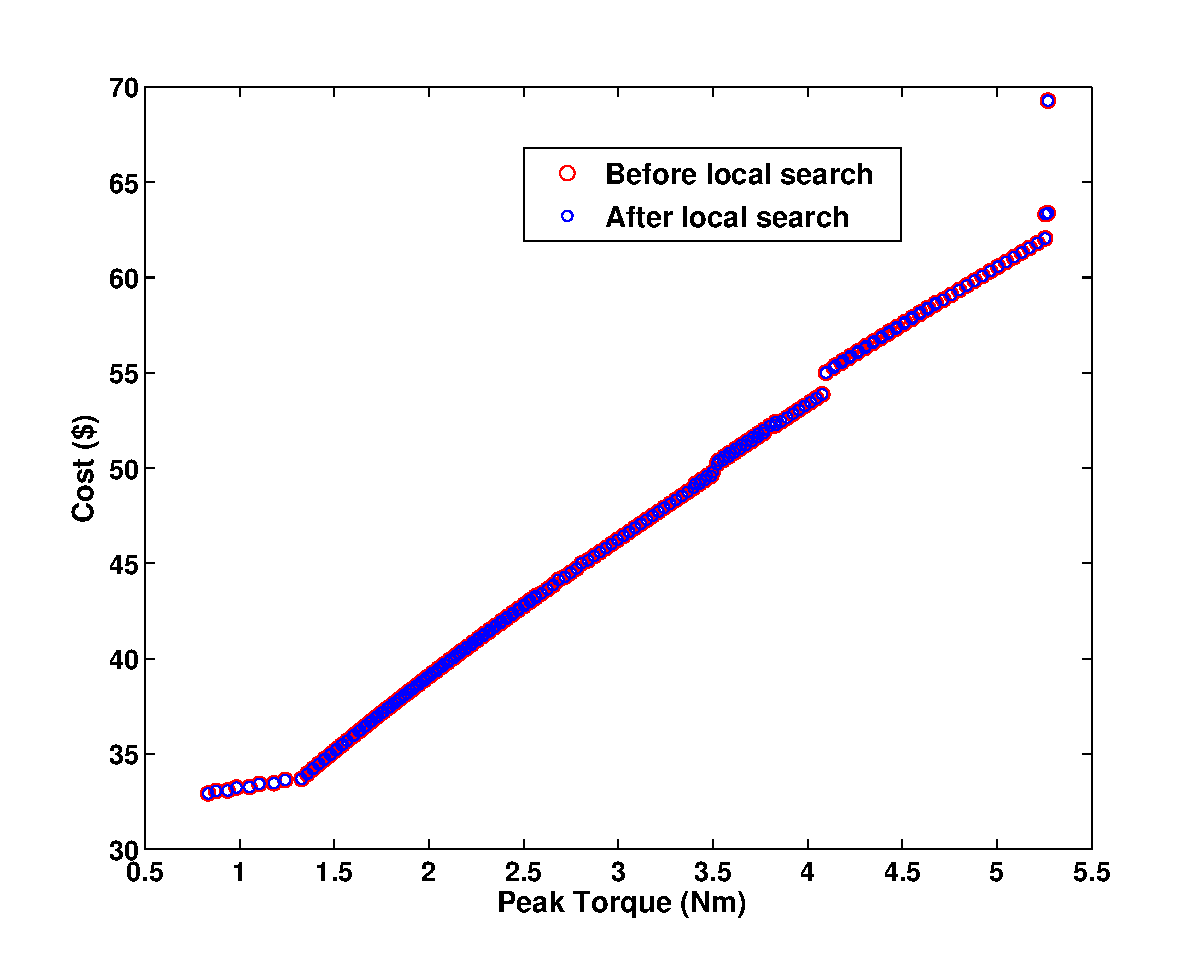
\includegraphics[width=90mm, height=75mm]{dia/nsplsp.eps} 
 \caption{Pareto-front for the BDCPMM design problem. The red circles represent the design results of NSGA-II and the blue circles represent the design results of the local search. Pareto-front obtained after the local search overlaps with the NSGA-II result.}
 \label{nsplsp}
\end{center}\end{figure}


\subsection{Local search procedure}
Although an evolutionary procedure may find a set of near optimal solutions
quickly, the convergence to the true pareto-front might take indefinitely
long. To improve convergence characteristics of the evolutionary
multi-objective algorithms they are often complemented with a local search
procedure. Local search is more important in case of multi-objective
optimization problems which involve discrete variables.  We have used a
generic local search procedure which evaluates random solutions in the
vicinity of the near-optimal solution under consideration. The input for
local search are the set of near optimal solutions $S$, number of local
search iterations to perform $n$, number of local solutions to evaluate for
each near optimal solution $h$, and the search width factor
$\sigma$. Algorithm \ref{localsearch} gives the pseudo-code for our local
search procedure.

\begin{algorithm}
  \SetKwInOut{Input}{input}\SetKwInOut{Output}{output}
  \Input{($S$, $n$, $h$, $\sigma$)}
  \Output{Set of optimal solutions $P$}
  $P = \phi$;\\
  \For{$i = 0$ to $n$}{
    \For{each $s \in S$}{
      add $s$ to $P$;\\
      find $k$ nearest neighbors of $s$;\\
      find the range of values each variable takes in the $k$-neighborhood;\\
      \For{$j = 0$ to $h$ }{
        generate a candidate random solution $p$ having variable values in the 
        neighborhood range scaled by $\sigma$;\\
        add $p$ to $P$;
      }
    }
    perform non-dominated sorting on $P$ and discard dominated solutions;\\
    $S$ = $P$;
  }
  return $P$;
  \BlankLine
  \caption{Local search procedure.}
  \label{localsearch}
\end{algorithm}

For the BDCPMM design problem, however, local search doesn't result in much
improvement since we ran NSGA-II for a large number of generations(3000)
which would have been sufficient for convergence to the actual
pareto-front. Performing local search on the NSGA-II output for BDCPMM
design problem increases the number of optimal solutions to 201 from 199.

\section{Estimating the pareto-front manifold}
We apply Isomap and PCA to estimate the dimensionality of the pareto-front
manifold and learn global properties of the set of the good designs. After
clustering this process will again be applied to the obtained chunks to
elicit the chunk local properties and capture their semantics.

% If $k$ conflicting objectives have to be optimised simultaneously in a
% multi-objective optimization, the resulting pareto-front would be a $k-1$
% dimensional manifold in the obejctive space. Modelling the pareto-front as
% a manifold may reveal how the objectives are related to each other, whether
% they are mutually conflicting in which case we will get a $k-1$ dimensional
% manifold, or some of them vary directly with each other, then the manifold
% will be of dimension less than $k-1$.  Similarly a linear dimensionality
% reduction analasys using PCA may reveal the relative importance of the
% decision variables in the optimal solutions.
  
\subsection{Isomap Residual Variance for the Pareto-front}
On performing Isomap on the pareto-front data of BDCPMM design we obtain a
residual variance plot shown in figure \ref{isoRVbdcpmAll}.  Since the
residual variance shows a sharp decline going from one dimensional
embedding to two-dimensional embedding, we can expect the pareto-front to
be composed of sub-manifolds of one or two dimensions.  There is an
unexpected increase in the residual variance for three dimensional
embedding, though it drops down to the previous level for four dimensional
embedding.

\subsection{PCA explained variance}
The PCA analysis of BDCPMM pareto-front gives four principal
components. The explained variance for principal components of the BDCPMM
pareto-front data are plotted in figure \ref{pcaEVbdcpmAll}.  The first
principal component has explained variance of more than 0.95, while the
second principal component has explained variance of 0.021.  The third and
fourth principal components have negligible explained variances. Table
\ref{first2BDPCs} shows the first two principal component vectors which
reveal that the pareto front is a manifold embedded in the plane of first
two design dimensions, namely number of laminations and number of turns in
the stator windings.
 

\begin{figure}[ht]\begin{center}
    \subfloat[Isomap Residual Variance.]{
      \label{isoRVbdcpmAll} \includegraphics[width=62mm, height=52mm]{dia/isoRVbdcpmAll.eps}}
    \subfloat[PCA Explained variance.]{
      \label{pcaEVbdcpmAll} \includegraphics[width=62mm, height=52mm]{dia/pcaEVbdcpmAll.eps}}
    \caption{Isomap and PCA results. The residual variance plot shows the
      largest drop for the second dimension indicating a manifold of
      dimension one. First principal component has an 95\% explained
      variance indicating a linear dimensionality of one.}
    \label{bdcpmmVar}
  \end{center}
\end{figure}

\begin{table}[!ht]
  \centering
  \begin{tabular}{c|c|c|c|c|c|}
    \cline{2-6}
    & $n_l$ & $N$ & $ L_{type} $  & $ M_{ph}$ & $a_{gauge}$ \\
    \hline
    \multicolumn{1}{|c|}{First PC} & 0.9993 & 0.0370 & 0.0072 & 0 & -0.0024\\
    \hline
    \multicolumn{1}{|c|}{Second PC} & -0.0367 & 0.9943 & 0.0165 & 0 & 0.0985\\
    \hline
  \end{tabular}
  \caption{First two principal components of the BDCPM data. Number of laminations is the dominant variable in the first principal component.}
  \label{first2BDPCs}
\end{table}


\section{Clustering the pareto-front}
Our chunking process aims to identify solutions with similar
characteristics and group them together. Those solutions of a
multi-objective optimization which are close together in the combined
objective-decision variables space, can be expected to have some shared
characteristics. Clustering the pareto-front is a way to group similar
solutions together.

\begin{figure}[ht]
  \begin{center}
    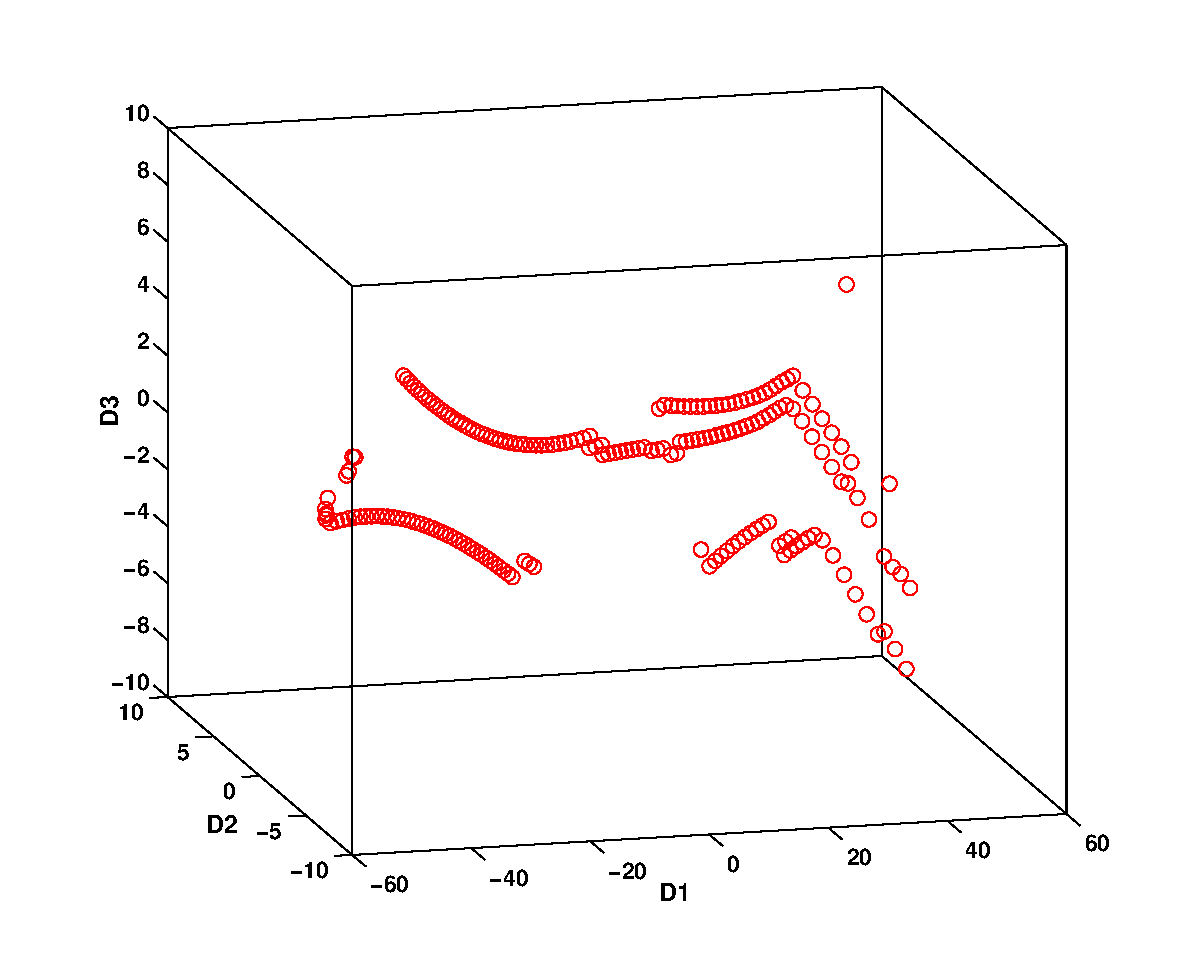
\includegraphics[width=90mm, height=75mm]{dia/bdcpmiso3.eps} 
    \caption{3-dimensional Isomap Embedding of the BDCPMM problem
      pareto-front, showing several one-dimensional manifolds.}
    \label{bdcpmiso3}
  \end{center}
\end{figure}

Figure \ref{bdcpmiso3} shows the 3-dimensional Isomap embedding of the
BDCPMM pareto-front. The embedding algorithm used in the Isomap is the
classical multi-dimensional scaling (cMDS), which aims to preserve the
inter-point distances in the reduced dimension. The 3-dimensional Isomap
embedding is thus an approximate modelling of the data set in the original
parameter space, with distances along the manifold preserved. This figure
clearly suggests that the BDCPMM pareto-front is composed of
one-dimensional manifolds, some of which run parallel to each other. Our
aim in clustering the pareto-front is to recover these lower dimensional
sub-manifolds.

We use an algorithm that is based on concepts of density-based partitioning
to cluster the pareto-fronts. One advantage of density based clustering is
that it is able to discover clusters of arbitrary shapes. DBSCAN is a major
representative of density based clustering.  DBSCAN works by identifying
\emph{core objects} in the data, those points in the data-set that have
at least $MinPts$ points within their $\epsilon$-neighborhoods. Two points
$x$ and $y$ have \emph{density connectivity} between them if there exists a
sequence of core objects between $x$ and $y$ such that each next belongs to
an $\epsilon$-neighborhood of its predecessor. Two points with density
connectivity between them belong to the same cluster. $MinPts$ and
$\epsilon$ are the only two parameters that this algorithm requires.

Our variant utilizes the concept of density connectivity, but we do not
attempt to explicitly identify the core objects. Instead, density
connectivity between points is determined by building a graph based on
density. Initially, all the points in the data-set are nodes in the
graph. We start by finding $n_{max}$ nearest neighbors of each point in the
data-set and sort these lists of nearest neighbors in the increasing order
of their distances from the point. At the beginning of each iteration, the
average edge weight ($ad_c$) and edge weight standard deviation
(${\sigma}_c$) are calculated for each component.  We connect each point
$p$ with the first point in its nearest neighbor list only if its distance
from the point is within $k{\sigma}_c + ad_c$ for the component $c$ to
which $p$ belongs, or else if average edge weight in the component is zero
($p$ is not connected to any other node), then average global inter-point
distance is used in place of $ad_c$. If an edge is added then the nearest
neighbor is popped from the list, otherwise we don't process $p$ in
subsequent iterations, as it means that either $p$ is an outlier or a
boundary point of the cluster. This process is repeated for $n_{max}$
iteration, by which time all the nearest neighbors lists will be empty. The
pseudo-code of the algorithm is shown in the listing \ref{clusteralgo}.

Our variant differs from DBSCAN in two important aspects. First, our
algorithm allows for clusters with different intra-cluster point densities,
since the decision that a point belongs to a cluster is based on its
distance from the nearest point in the cluster, and the average edge weight
within the component.  DBSCAN may fail to identify a cluster with lower
point density because of a low $\epsilon$ parameter. Secondly in place of
the $\epsilon$ parameter we have $n_{max}$ parameter giving the number of
nearest neighbors that must be found for each point. The number and size of
clusters depends on the parameter $k$.


\begin{algorithm}
  \SetKwInOut{Input}{input}\SetKwInOut{Output}{output}
  \Input{($D$, $n_{max}$, $k$)}
  \Output{A cluster labelling for each data-point}
  \BlankLine
  find $n_{max}$ nearest neighbors of each point arranged in non-decreasing
  order of the distance;\\
  $ad_{g} =$ average inter-point distance in the data set;\\
  ${\sigma}_g =$ standard deviation of distances in the data set;\\
  $G =\{V, E\}$ be a graph where $V$ is the set of all data-points and $E = \phi$;\\ 
  \For{$i = 1$ to $n_{max}$}{
    \For{each connected component $c$ in $G$}
    {
      find out the average and standard deviation of edge weights in $c$;\\
    }
    \For{each point $p$ in the data set}
    {
      \If{ $p$'s nearest neighbor list is empty}
      {
        continue;\\
      }
      $c =$ component label of the component $p$ belongs to; \\
      $q =$ the first point in the nearest neighbor list of $p$;\\
      $d =$ distance to first point in ordered nearest neighbors list of $p$;\\
      \eIf{i = 0}
      {
        $thresholdDistance = ad_g + k {\sigma}_g$ ;\\
      }
      {
        $thresholdDistance = ad_c + k {\sigma}_c$ ;\\
        \tcc{$ad_c$ and ${\sigma}_c$ are the average and standard deviations of edge weights in $c$}
      }
      
      \eIf{$d > thresholdDistance$}
      {
        \tcc{if $i = 0$ then $p$ is either an outlier or boundary}
        remove all points from the ordered nearest neighbors list of $p$;\\
      }
      {
        \If{ $(q, p) \notin E$}
        {
          add ($p$, $q$) to $G$;\\
          remove $q$ from ordered nearest neighbors list of $p$;\\
        }
      }
    }
  }
  label points in $V$ with the component they belong to; \\
  return $V$;\\
  
  \caption{Clustering algorithm to obtain low-dimensional clusters}
  \label{clusteralgo}
\end{algorithm}


The clustering of the BDCPMM pareto-front results in five clusters which
are shown in the objective space plot in figure \ref{bClustersO}.  Figure
\ref{bClustersP} shows the clusters with respect to the number of
laminations ($n_l$) and the number of turns ($N$) in the stator windings.
Other design variables are indicated alongside the clusters.

\begin{figure}[ht]
  \begin{center}
    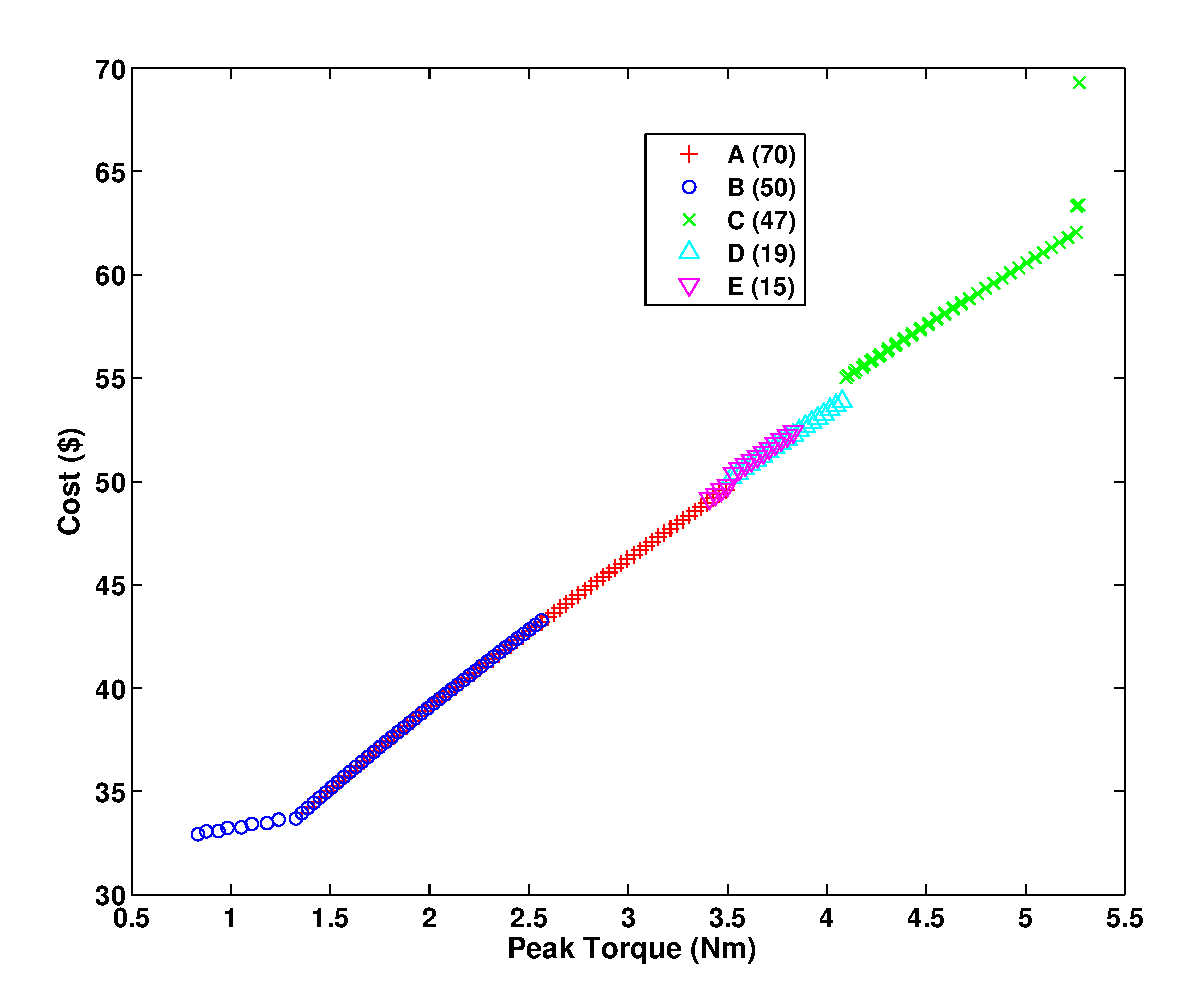
\includegraphics[width=100mm, height=80mm]{dia/bClustersO3.eps} 
    \caption{Clusters in the BDCPMM pareto-front. Clusters \textbf{A} and
      \textbf{B} are composed of low power and cost designs while Cluster
      \textbf{D} as the high-power and cost designs.}
    \label{bClustersO}
  \end{center}
\end{figure}

\begin{figure}[ht]
  \begin{center}
    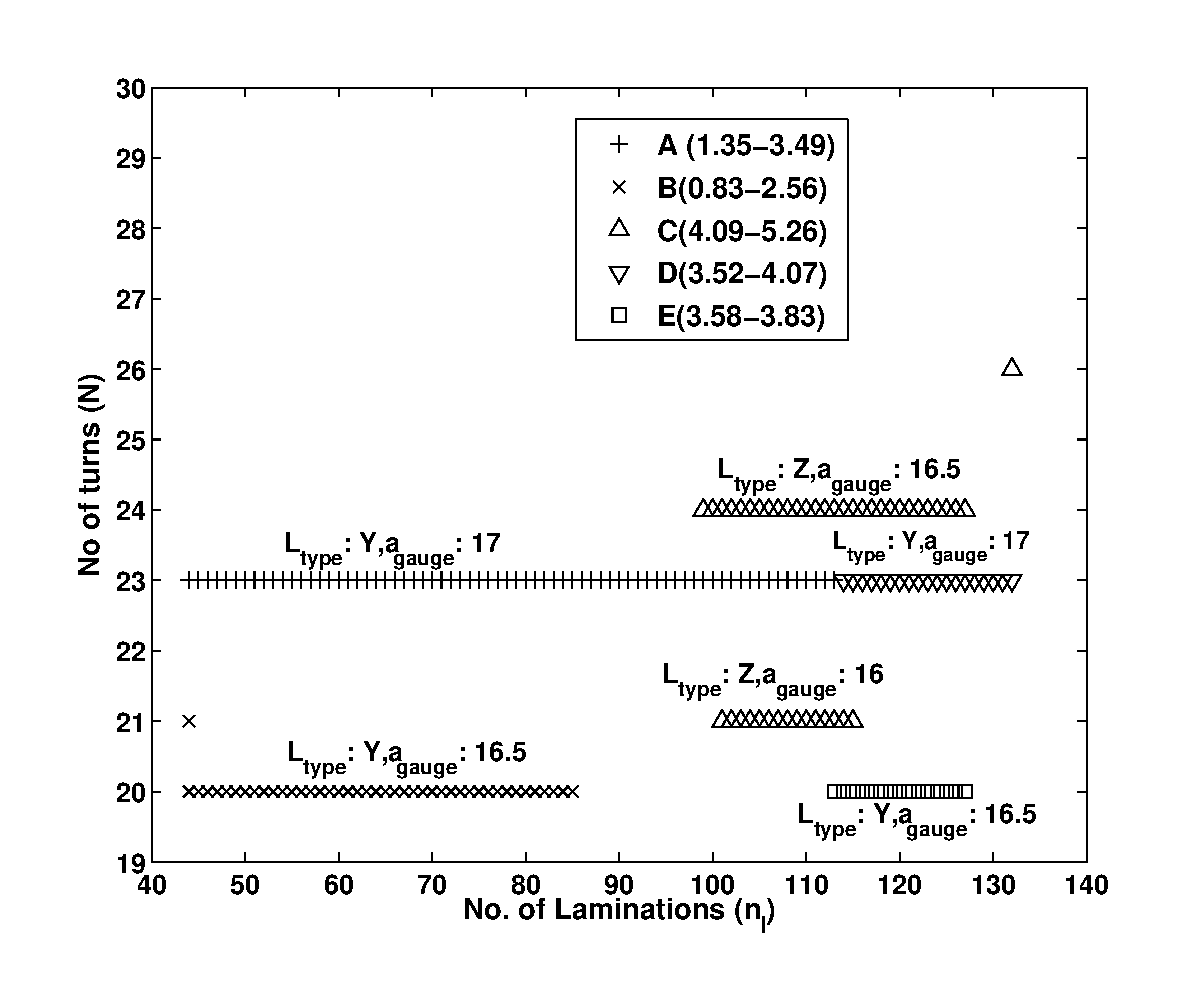
\includegraphics[width=100mm, height=80mm]{dia/bclustersp3.eps} 
    \caption{Clusters in the $n_l$-$N$ subspace. All the clusters appear as
      lines in the parameter space except the cluster of high-end designs
      \textbf{D} which appears as two separate lines.}
    \label{bClustersP}
  \end{center}
\end{figure}
 
\section{Manifold modelling of the clusters}
In this step we apply manifold learning and linear dimensionality reduction
to the clusters obtained in the previous step in an attempt to uncover the
nature of the clusters. We again use Isomap to uncover the shape and
dimensionality of each cluster and PCA to elicit shared design
characteristics of solutions in each cluster. However, since the clusters
may be linear patches of the whole manifold, PCA analysis reveals more
useful information than Isomap analysis. All the clusters except \textbf{C}
have negligible or zero residual variance for one dimensional Isomap
embedding, indicating that they are one-dimensional.  Residual variances
for \textbf{C} are plotted in figure \ref{bClusterCrv}. The residual
variance shows a large drop from two dimensional Isomap embedding to three
dimensional Isomap embedding, after which it is flat. This means that
cluster \textbf{C} has intrinsic dimensionality of two. Looking at figure
\ref{bClustersO} and \ref{bClustersO} reveals why it is so. The cluster
\textbf{C} has higher torque motors, but unlike other clusters which have
the same number of turns in the stator windings, it has two types of
designs with 21 and 24 turns. The wire gauges are also distinct in these
two types of designs, those with 21 turns use 16 gauge wire and those with
24 turns use 16.5 gauge wire.

These findings are in accordance with the {\em chunk dimensionality
  conjecture} proposed in section \ref{cdc}, whereby chunks are manifolds
in the decision space of dimensionality less than the dimensionality of the
decision space. The dimensionality of these manifolds in the decision space
is also less than or equal to the dimensionality of the objective space,
which is two in this case. Four clusters have manifold dimensionality of
less than two and only one has two dimensions.

 
\begin{figure}[ht]
  \begin{center}
    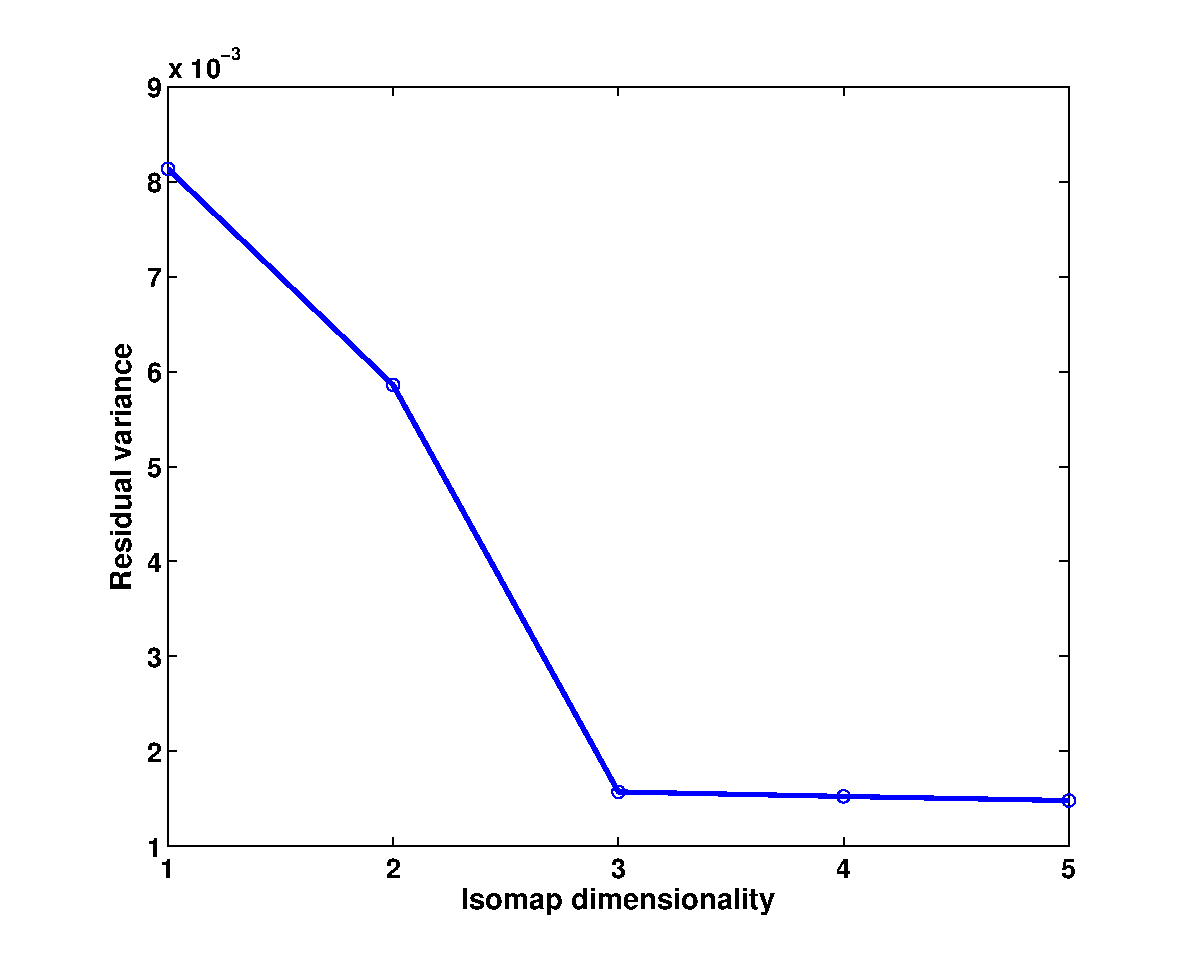
\includegraphics[width=60mm, height=50mm]{dia/bclusterCrv.eps} 
    \caption{Residual variance for the cluster \textbf{C}. The largest drop
      in the residual variance is for the 3-dimensional Isomap embedding,
      indicating a two dimensional manifold.}
    \label{bClusterCrv}
  \end{center}
\end{figure}

Table \ref{clustersEV} shows the explained variances for principal
components of each of the clusters. The explained variances corroborate the
observations made in the Isomap analysis that four of the clusters are one
dimensional and only one cluster (\textbf{C}) is two dimensional. Table
\ref{clusterPC} lists the first principal components of the clusters
\textbf{A}, \textbf{B}, \textbf{D} \textbf{E}. Since cluster \textbf{C} is
two dimensional, its two principal components are shown.

\begin{table}[!ht]
  \centering
  \begin{tabular}{|c|c|c|c|c|c|}
    \hline
    \textbf{A} & 100 & 0 & 0 & 0 & 0 \\
    \hline
    \textbf{B} & 99.857 & 0.119 & 0.02 & 0 & 0\\
    \hline
    \textbf{C} & 70.82 & 29.17 & 0.01 & 0 & 0\\
    \hline
    \textbf{D} & 100 & 0 & 0 & 0 & 0\\
    \hline
    \textbf{E} & 100 & 0 & 0 & 0 & 0\\
    \hline
  \end{tabular}
  \caption{Explained variances for the principal components of the clusters. For clusters \textbf{A}, \textbf{B}, \textbf{D} and \textbf{E} there is only one significant principal component. Cluster \textbf{D} has two significant principal components.}
  \label{clustersEV}
\end{table}

\begin{table}[!ht]
  \centering
  \begin{tabular}{c|c|c|c|c|c|}
    
    \cline{2-6}
    & $n_l$ & $N$ & $ L_{type} $  & $ M_{ph}$ & $a_{gauge}$ \\
    \hline
    \multicolumn{1}{|c|}{\textbf{A}} & 1 & 0 & 0 & 0 & 0 \\
    \hline
    \multicolumn{1}{|c|}{\textbf{B}} & 0.999 & 0.0077 & 0 & 0 & -0.019\\
    \hline
    \multicolumn{1}{|c|}{\multirow{2}{*}{\textbf{C}}} & 0.789 & 0.610 & 0 & 0 & 0.066\\ \cline{2-6}
    \multicolumn{1}{|c|}{}& -0.613 & 0.785 & 0 & 0 & 0.074\\
    \hline
    \multicolumn{1}{|c|}{\textbf{D}} & 1 & 0 & 0 & 0 & 0\\
    \hline
    \multicolumn{1}{|c|}{\textbf{E}} & 1 & 0 & 0 & 0 & 0\\
    \hline
  \end{tabular}
  \caption{Principal components for the clusters. For \textbf{A} \textbf{B} \textbf{D} and \textbf{E} the principal component is along the direction of $n_l$. Cluster \textbf{C} has two components which are in the $n_l - N$ plane. }
  \label{clusterPC}
\end{table}

\section{Design implications}
There are a number of important facts that can be observed from the PCA
analysis of the clusters. Firstly, as is evident in the tables
\ref{first2BDPCs} and \ref{clusterPC}, number of laminations is the most
important design parameter, as this is the variable that has the largest
weights in the first principal component of the whole pareto-front and the
clusters. This parameter can be changed for inducing a small amount of
change in the peak torque and cost.

The connection type ($M_{ph}$) has no contribution whatsoever in the
principal components of the pareto-front and the clusters. This means that
all the optimal designs must be using the same connection type. Only
\emph{Y} connection type is used in all the designs.
 
Although the variable $L_{type}$ has no weight in the principal
components of the clusters, it has some contribution to the principal
component of the overall pareto-front. This means that lamination type is
the same for all the designs in a single cluster, though it may vary across
the pareto-front. Only two out of three lamination types are used in all
the designs. Lamination type Y is used in all the clusters except
\textbf{C}, in which lamination type Z is used.  Looking at figure
\ref{bClustersP} we can see that cluster \textbf{C} occupies the highest
torque and cost range of the pareto-front. This implies that lamination
type Z is only useful for high end designs of BDCPM motors.

Number of turns ($N$) has a small weights in the principal components of
the pareto-front. The principal components of clusters \textbf{A},
\textbf{D} and \textbf{E} have zero weights for $N$, and \textbf{B} and
\textbf{C} have non-zero weights. Incidentally, these are also the only
clusters that have non-zero weights for the variable $a_{gauge}$. This
suggests that these two variables are not independent of each other in the
optimal designs. The number of turns tend to stick to the lower region
(20--24) of the range of possible values (20--80). Also higher
cross-section wires (lower $a_{gauge}$) among the available choices are
used in the optimal designs

\section{How the chunks relate to experts' intuition}
\label{bdcpmDiscuss}
The observations made in the previous section are in confirmation of the
expert's intuition of the design of a BDCPM motor, discussed in the section
\ref{expertInAction}. To the expert it was `natural' that if higher peak
torque is desired then number of laminations have to be increased
proportionately. Increasing the number of turns in the stator winding also
increases the torque, but in much larger quanta's. Also, since
non-customizable lamination designs are used, it may not be possible to
increase the number of turns, the reason being that the size of the groove
($d_3$ in figure \ref{bdcpmStator} and table \ref{ltypeDimTable}) that
accommodates the windings is fixed for each lamination type. So to increase
the number of turns either a lamination type with larger radial dimensions
must be used or a wire with smaller cross-section must be chosen for the
windings.

All these trade-offs can be clearly observed in play in the cluster of
high-end designs (\textbf{C}) where the lamination type with largest radial
dimension is used and two combinations of number of turns and wire
cross-section are employed. One set of designs has 21 turns with 16 gauge
wire and the other has 24 turns with 16.5 gauge wire.


When the expert had to choose the connection type in the winding, he chose
the {\em Y} type connection, although reasons for the choice were not
immediately clear. After some back of the envelop calculations, the
explanation he gave was that since the wire cross-section is fixed, the
maximum current that can flow in the stator winding is limited and {\em Y}
connection type allows for a higher power factor. Indeed, all the optimal
designs in our results have a {\em Y} connection type.
